\section{Experiment}
\subsection{Problem Statement}
Given multiple EEG signals from a set of interconnected neuronal regions, can the CCM model identify structural patterns in causal relationships between those regions? Can the patterns and properties of the causality graph resulting from the CCM model be clustered into brain states that represent different stages of epilepsy in the brain? In other words, can a machine learning algorithm be applied to the causal network properties, the model of which could be able to correctly classify epileptic brain states.

\subsection{Methods}
\subsubsection{Data Collection}
EEG data was collected from an 4x8 endodermal electrode array at a frequency of 1000 Hz (31 channels, one channel malfunctioned, Fig. \ref{fig:rat_experiment}). The data recording lasts for ~500 seconds, during which epileptic seizures were evoked using 4-aminopyridine and EEG data was recorded from the electrode array. The spiking voltage of each recorded electrode is used as a signal and is referred to as a channel (Fig. \ref{fig:example_eeg_and_kcsd}). Each channel has a continuous data series that spans the 500 seconds.

\begin{figure}[H]
  \centering
  \begin{subfigure}[b]{0.45\textwidth}
    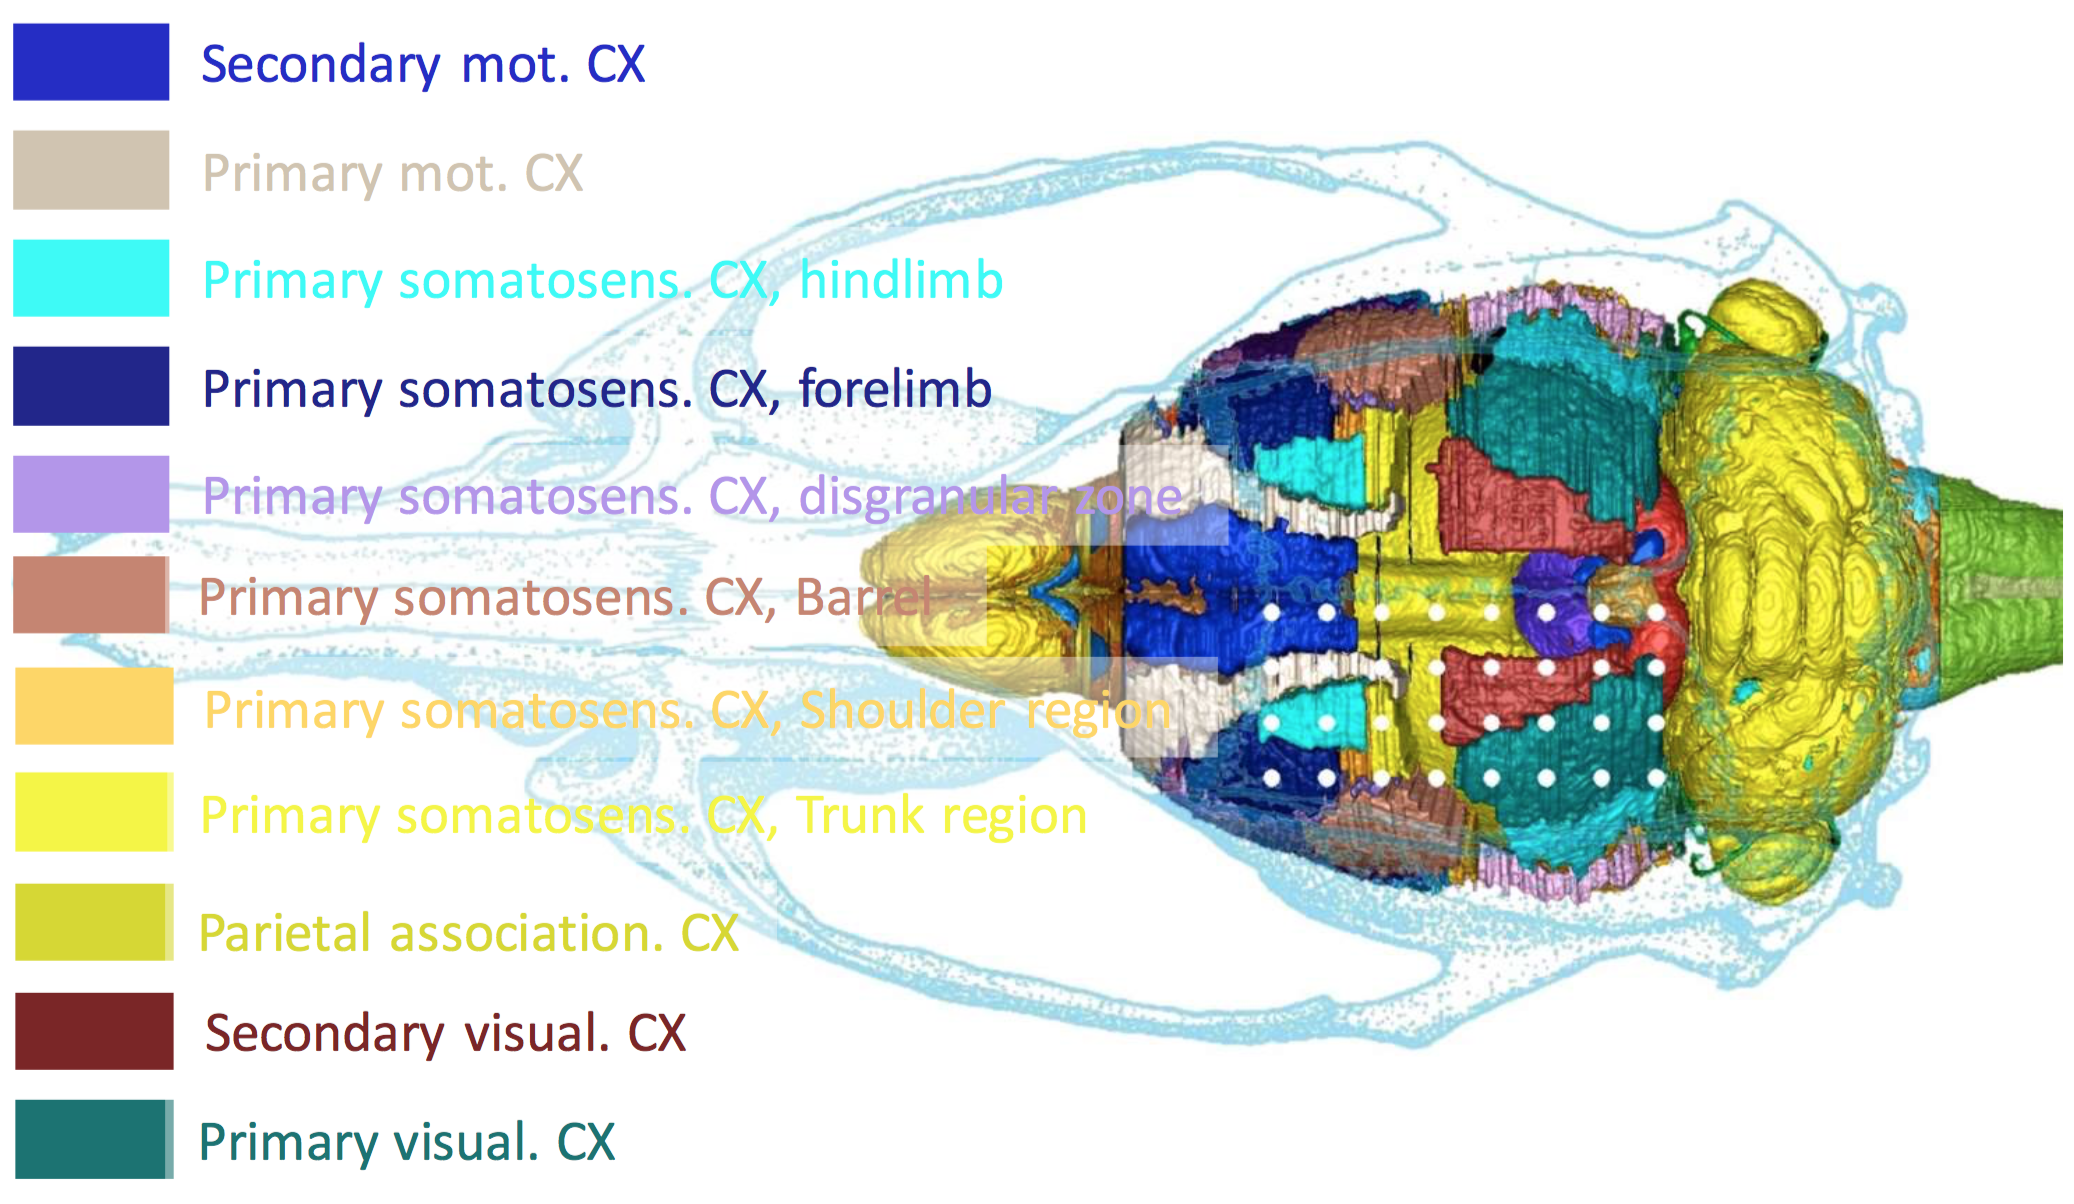
\includegraphics[width=0.95\linewidth]{figures/rat_brain_schematic.png}
    \caption{}
  \end{subfigure}
  \begin{subfigure}[b]{0.45\textwidth}
    \centering
    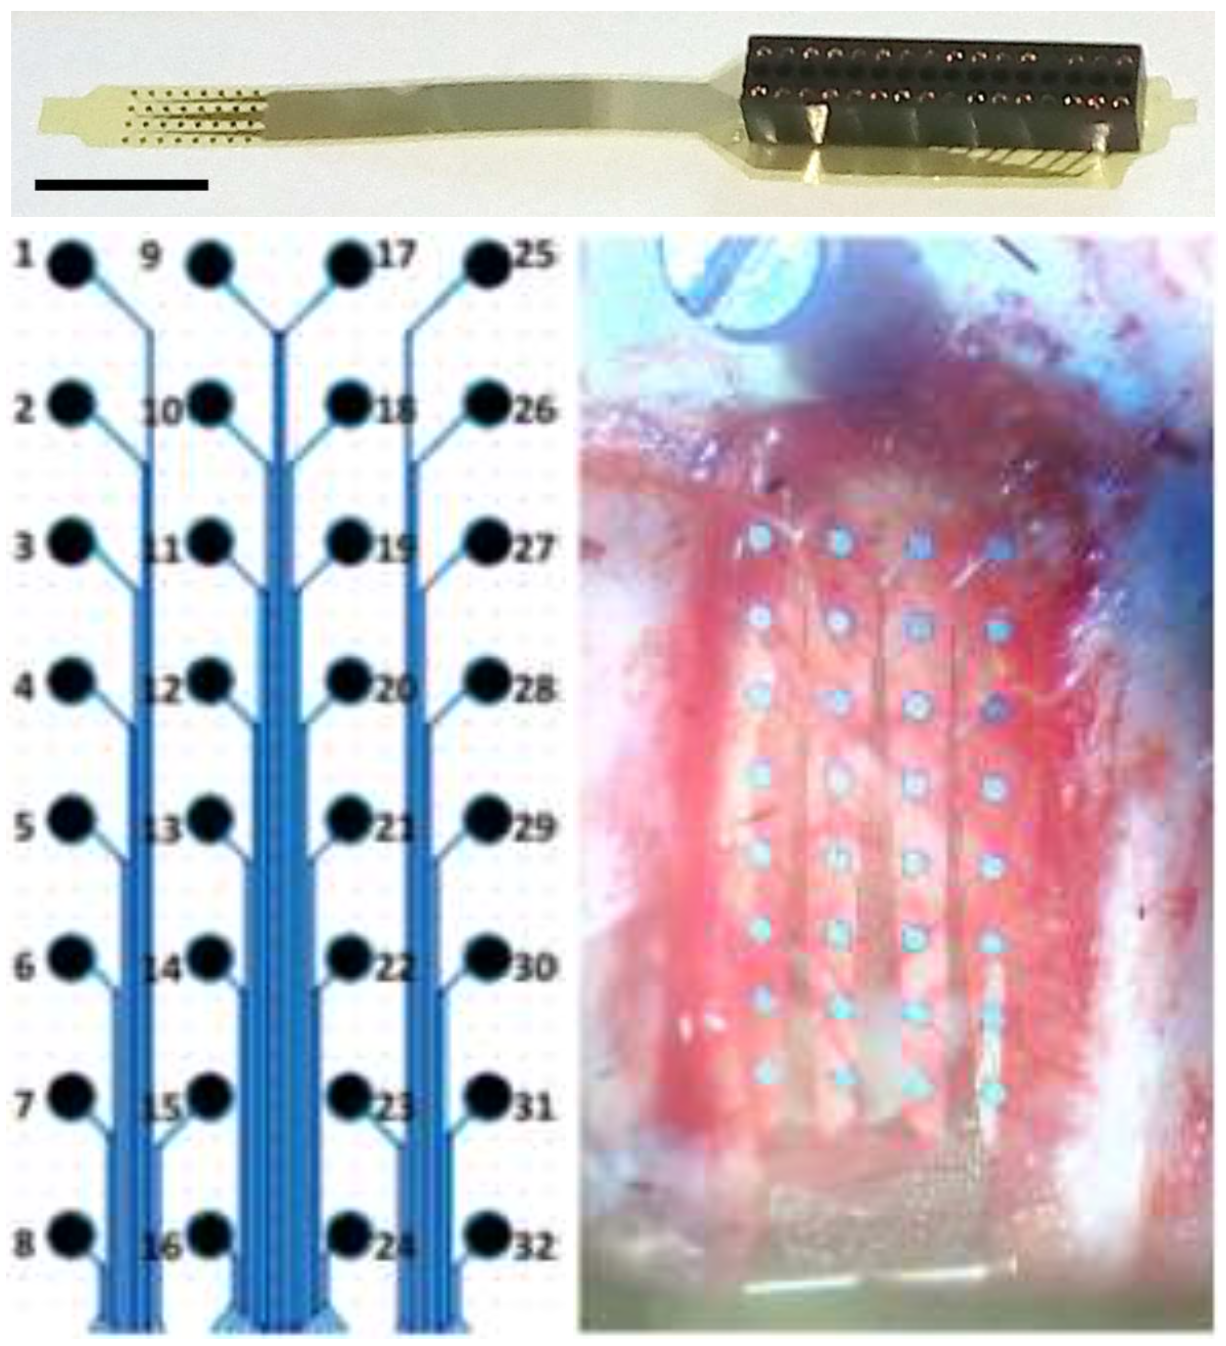
\includegraphics[width=0.95\linewidth]{figures/rat_scull_and_instrument.png}
    \caption{}
  \end{subfigure}
  \caption{(a) A composite drawing showing the brain in the scull. The 3D reconstruction of the brain has been made using the maps of the Paxinos atlas, and the localization of cortical areas are indicated by different colors. White points indicate the position of the recording sites of the membrane electrode. Names for the cortical areas are also shown (based on Hjornevik \textit{et al.} and Paxinos \textit{et al.} \cite{hjornevik2007} \cite{paxinos2009}). (b) Photograph of a membrane electrode shows the construction on the top, the numbering (bottom right) and the surgical implantation (bottom left) is also shown. Electrode 1 malfunctioned during recording.}
  \label{fig:rat_experiment}
\end{figure}


\begin{figure}[H]
  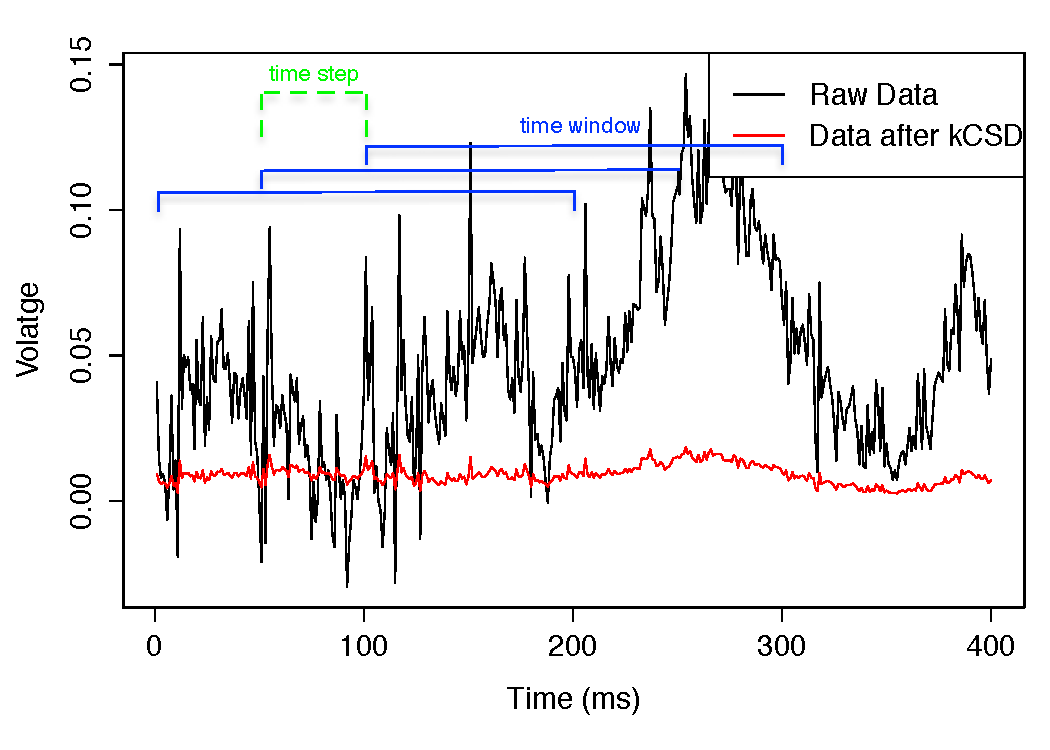
\includegraphics[width=\linewidth]{figures/sample_eeg_signal_with_kcsd_edited.pdf}
  \caption{Sample data from electrode 1, in both its raw form and then in its form after kCSD transformation. Applying kernel Current Source Density extracts the true relationship of neural activity, and in theory eliminates disturbances that might be caused by signal interference. Three sample blue lines are drawn to demonstrate the sliding windows that were used to calculate Sugihara Causality between brain regions. In each time window, the causality was calculated between each brain region, and the time window was moved by an amount \textit{time step}. Different configurations were used for the time window and time step, as reported in table \ref{tab:sliding_window_configuration}. Here, the configuration shown has time window as $200$ and time step as $50$.}
  \label{fig:example_eeg_and_kcsd}
\end{figure}

\begin{table}[H]
\centering
\caption{Configurations used for the sliding window when calculating Sugihara causality that was used as a measure of brain communication. These configurations inform our model of the granularity of brain communication. Since we do not know exactly how quickly information is being passed down from region to region, arbitrary choices were made to test how well each performs and make a more informed decision in future research. Because we have different time steps, there are a different number of graphs (data points) in each dataset.}
\label{tab:sliding_window_configuration}
\begin{tabular}{|c|c|c|c|}
\hline
 Dataset name &  Time window &  Time step & Number of Data points\\ \hline
 
 dataset 50 & 200 & 50 & 10190 \\ \hline
 dataset 200 & 200 & 200 & 2547 \\ \hline
 dataset 250 & 2000 & 250 &  2038 \\ \hline
\end{tabular}
\end{table}

\subsubsection{EEG Data Preprocessing}
Kernel Current Source Density (kCSD) method was used on the grid of channels to account for possible electrical interference with the direct measurement (Fig. \ref{fig:example_eeg_and_kcsd}) \cite{Potworowski2012}. The measured potentials produced by kCSD arise as the linear combination of the trans-membrane currents, which is a more direct and localized quantity to measure the neural activity. Therefore current source density distribution was calculated by the kCSD method and used for the analysis instead of the original EEG signals.

Afterwards, in order to reduce the data size that is operated on, we lumped channels from the same brain regions together by averaging them (Fig. \ref{fig:brain_region_lumping}). In addition to reducing dimensionality, this process also puts emphasis of causality on functional brain regions instead of a local cluster of neurons. 

\subsubsection{Sugihara Causality Measurement}
After lumping the kCSD signals from the same region, we perform Sugihara Causality calculation on the regions by using a sliding windows method (Fig. \ref{fig:example_eeg_and_kcsd}). Because we do not know how granular of a time frame the brain uses to communicate (and how that affects the EEG signal we record), we use three different time scales as reported in table \ref{tab:sliding_window_configuration}. This produces 3 datasets with similar characteristics. The important thing to keep in mind is that after this step, each causality measure that resulted from the Sugihara Causality analysis is a measure of how much one region is affecting the other, and we use that as a way to describe brain communication and information flow. Each causality measure is therefore an \textit{edge} of communication from one region to another, meaning that each brain region is a node and each causality measure is a weighted edge. Figure \ref{fig:sample_graph} shows a sample graph constructed from joining all the causality measures from a specific time window. This is essentially a (theoretical) snapshot of how each brain region was affecting other brain regions in that time window.

\begin{figure}[H]
  \centering
  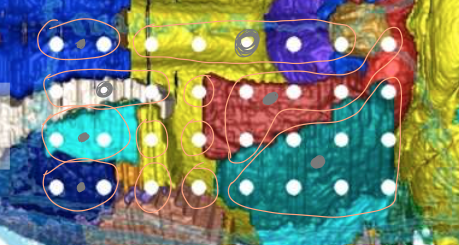
\includegraphics[width=0.65\linewidth]{figures/brain_region_lump.png}
  \caption{The distribution and lumping of the brain regions in the brain. A total of 12 region channels were constructed from the initial 31 local channels. The schematic is based on rat brain atlas mapping.}
  \label{fig:brain_region_lumping}
\end{figure}


\begin{figure}[H]
  \centering
  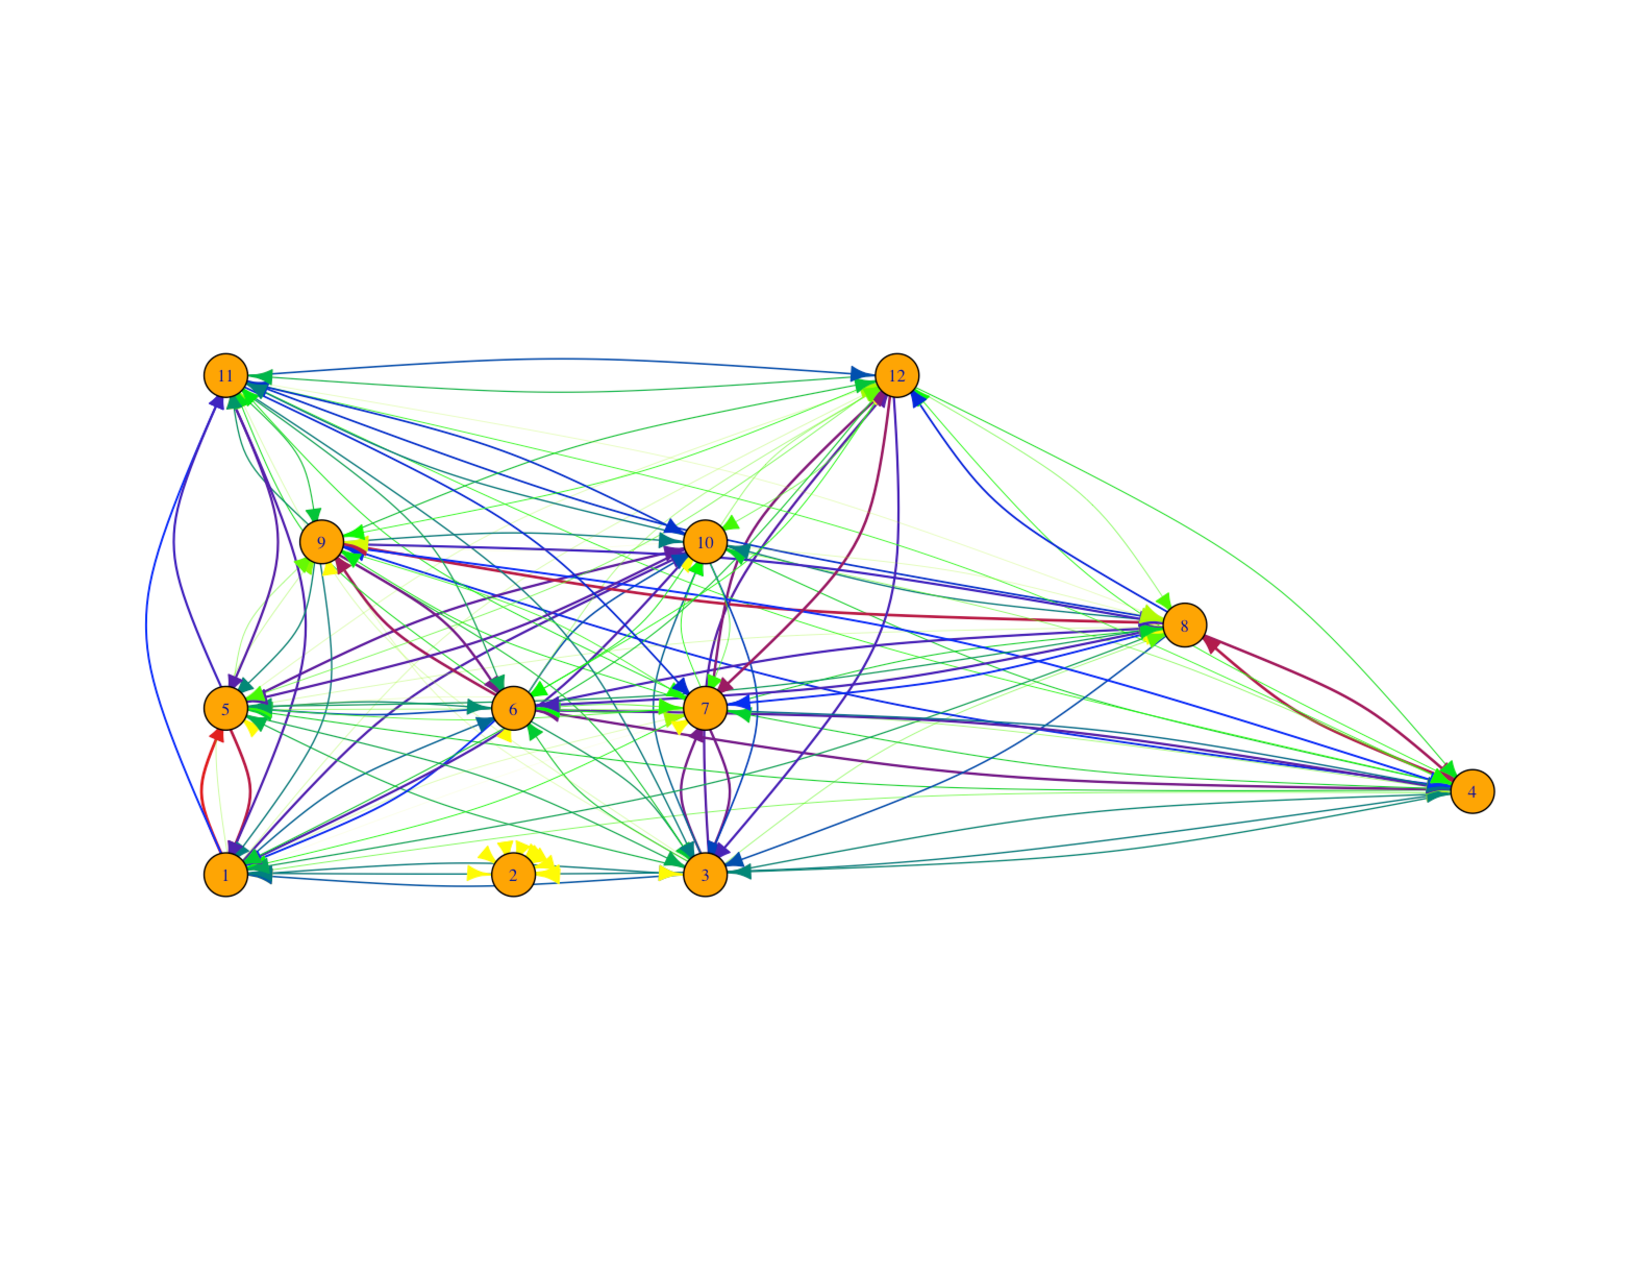
\includegraphics[width=0.55\linewidth]{figures/sample_graph.pdf}
  \caption{Sample graph constructed from calculating the Sugihara causality between brain regions. Lumped brain regions correspond to the gray circular mapping in Fig. \ref{fig:brain_region_lumping}. Edge colors represent the strength of the causal relationship. From weakest to strongest: Yellow, Green, Blue, Red. The edge weight ranges from 0 to 1.}
  \label{fig:sample_graph}
\end{figure}


\subsubsection{Data Exploration and Visualization}
The data we produced is a series of complete, directed graphs (all the same topology; each node is a brain region as seen in figure \ref{fig:rat_experiment}; each edge is a causality/communication measure) and their edge weights that we refer to as $\rho$ scores ($\rho$ is the convention name for the score of a Sugihara Causality analysis). Since we processed the data with different time steps, there are a different number of graphs available in each dataset (Tab. \ref{tab:sliding_window_configuration}). For each graph, there are $132$ $\rho$ scores, all of which range between 0 and 1 (decimals). Each graph was transformed into a vector where each vector is a data point, and all vectors make a dataset. This transformation was required for the data to be entered into sklearn's Gaussian Mixture model function properly.

In all graphs, most of the $\rho$ scores appear to be of high values, suggesting high connectivity between brain regions and therefore a high density graph (Fig. \ref{fig:rho_hist_all_experiment}). This indicates that there is constant information flow between regions in the brain. Furthermore, we also notice that many of the $\rho$ scores to be similar within a pair of nodes (Fig. \ref{fig:diff_within_pair_hist}). For example, when looking at regions 1 and 2 within the first 200 milliseconds, they appear to be equally communicating to one another (Fig. \ref{fig:sample_pair_causality_plot}). This could be indicative of either bidirectional causality or unidirectional forcing, both of which can be detected by the Sugihara model.

\begin{figure}[H]  
  \centering
  \begin{subfigure}{0.45\textwidth}
    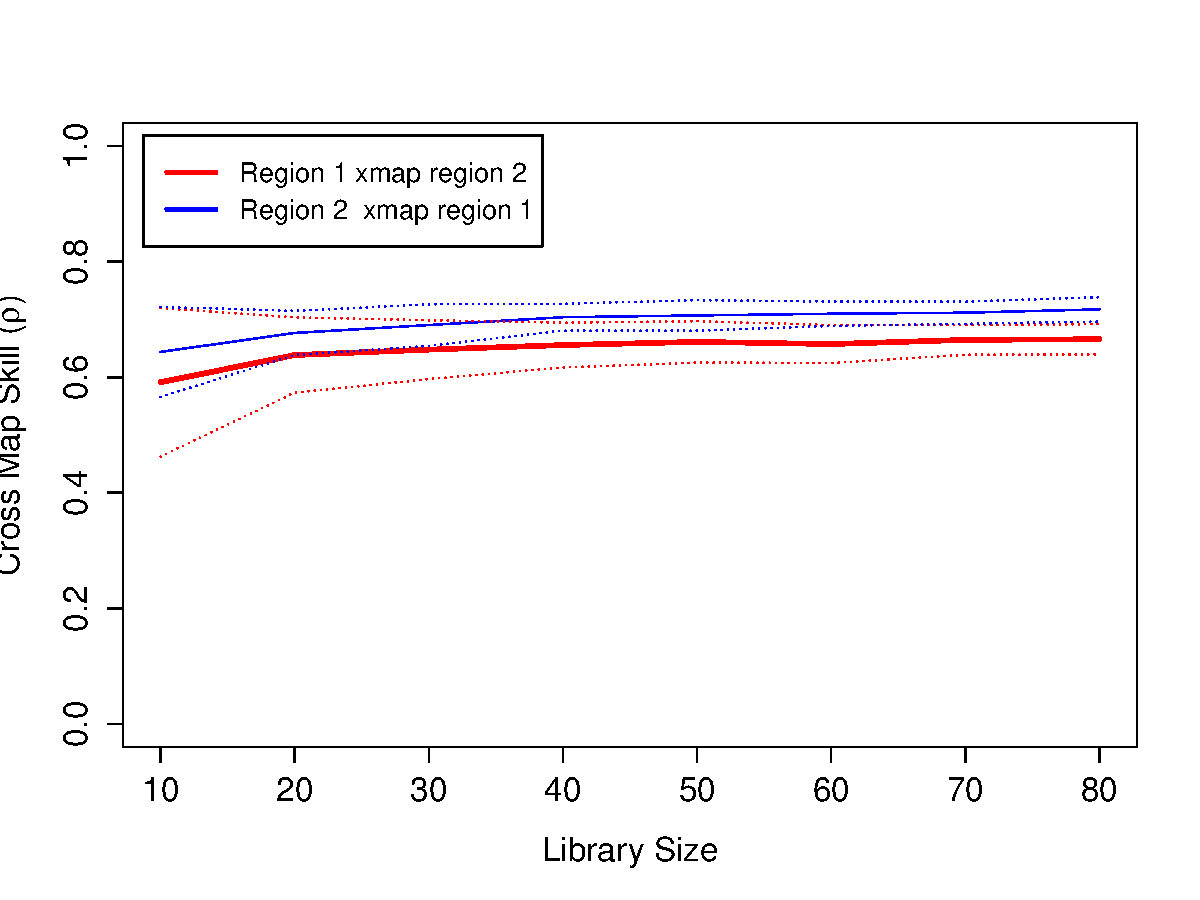
\includegraphics[width=\linewidth]{figures/sample_pairwise_causality_measure.pdf}
    \caption{}
    \label{fig:sample_pair_causality_plot}
  \end{subfigure}
  \begin{subfigure}{0.45\textwidth}
    \centering
    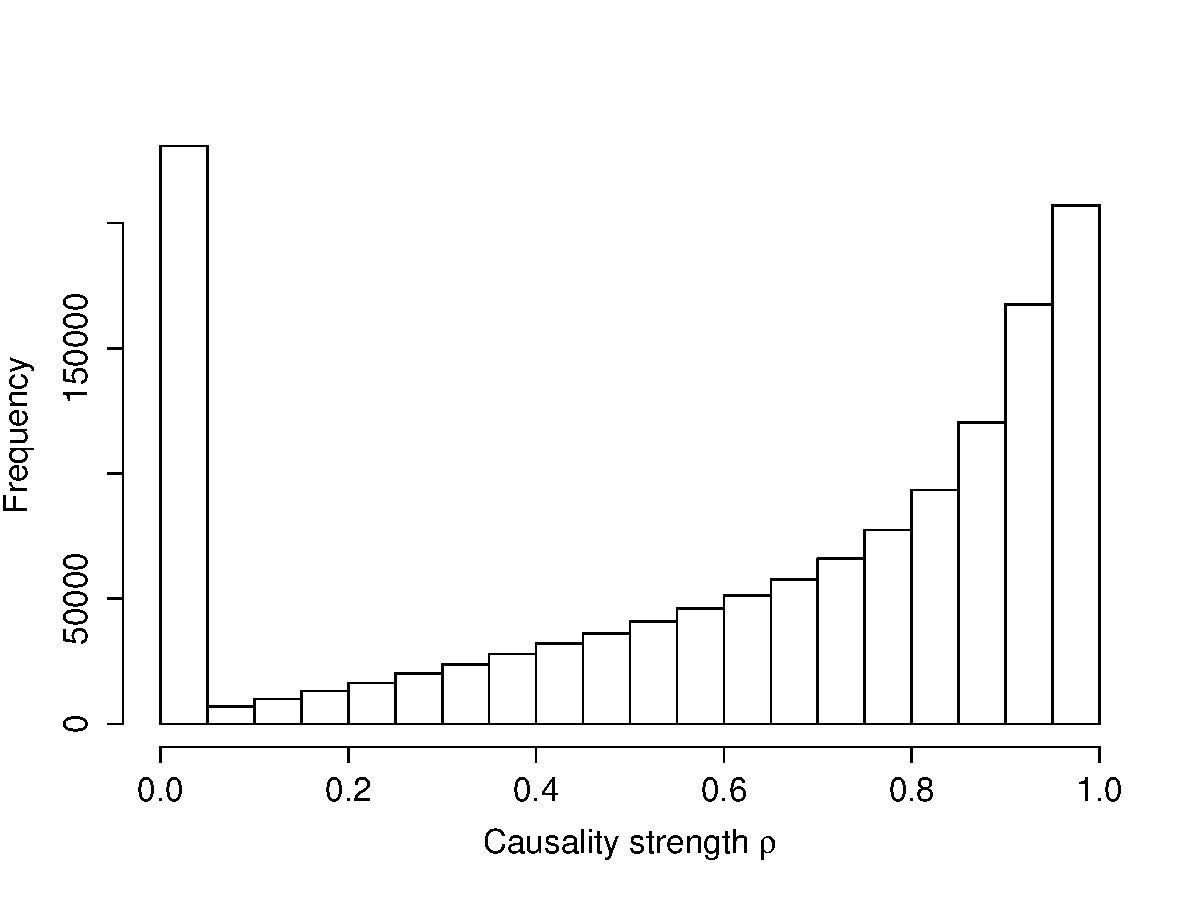
\includegraphics[width=1\linewidth]{figures/rho_hist_all_experiment.pdf}
    \caption{}
    \label{fig:rho_hist_all_experiment}
  \end{subfigure}
  \caption{(a) A sample graph plotting the convergent cross mapping skill ($\rho$) between region (nodes) 1 and 2 during the first 200 ms of the experiment. The skill mapping channel 1 to channel 2 is very similar to the one mapping channel 2 to channel 1. This might infer either bidirectional causality or unidirectional forcing. A similar pattern (close $\rho$ value between pairs) was found for most of the pairs of edges. (b) The distribution of CCM skill ($\rho$) during the entire experiment. Many relationships appear to be causal in the brain, with equally as many being non-causal throughout the experiment. Causality was calculated from signals of lumped regions after calculating the CSD. Cross mapping was done on every pair of regions with library size of 80, and each pair has two causality directions. Sliding windows of 200 ms were used, with a sliding step of 50 ms.}
\end{figure}

\begin{figure}[H]
  \begin{subfigure}{.48\textwidth}
    \centering
    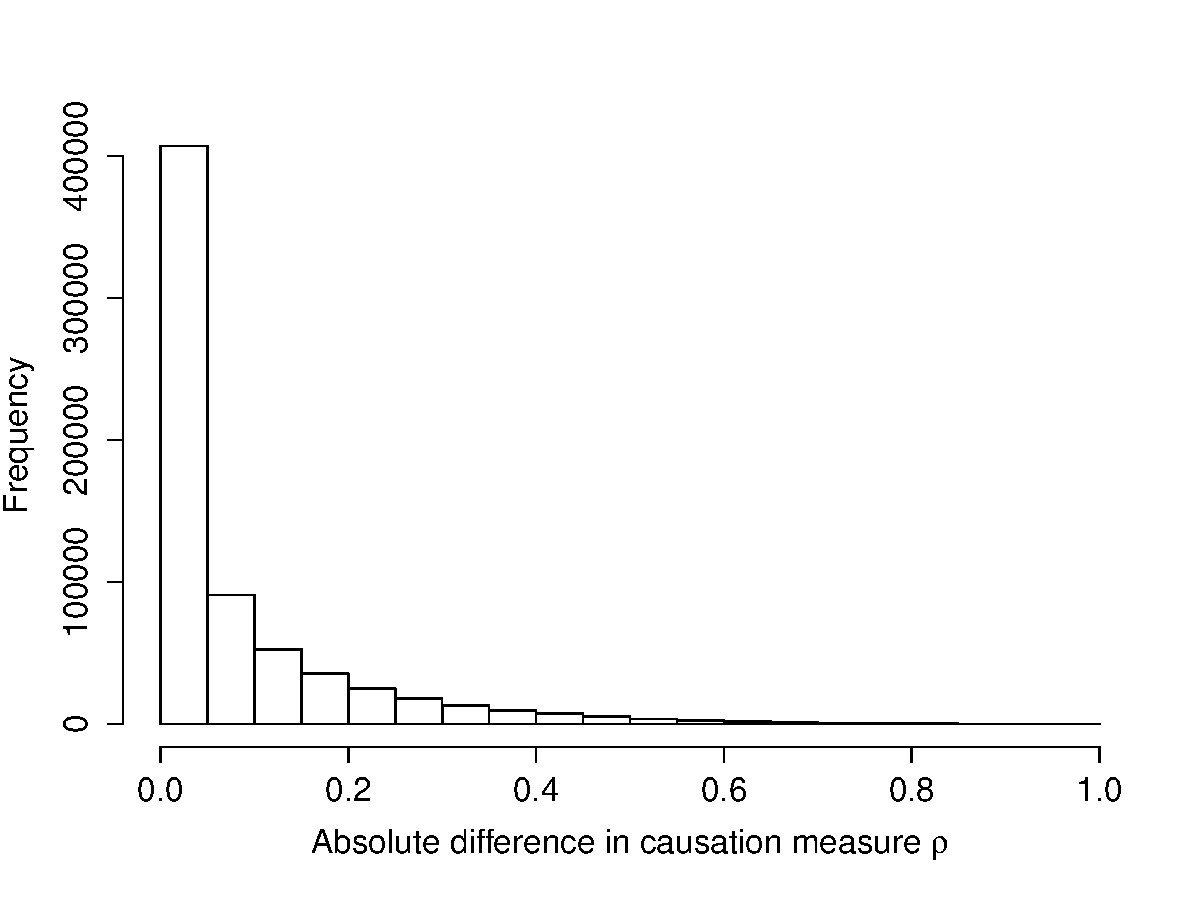
\includegraphics[width=0.95\linewidth]{figures/diff_within_pair_hist.pdf}
    \caption{Absolute difference of $\rho$ between all pairs}
  \end{subfigure}  
  \begin{subfigure}{.48\textwidth}
    \centering
    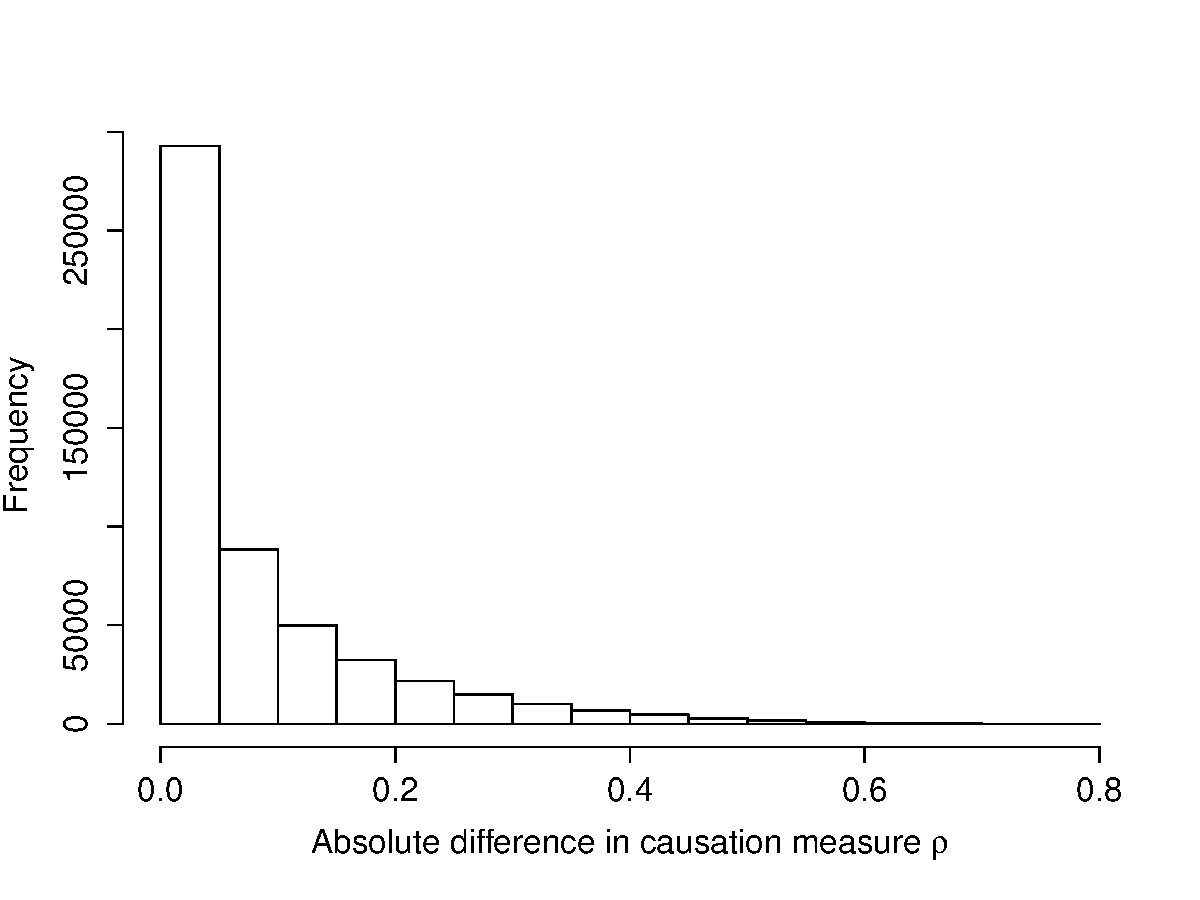
\includegraphics[width=0.95\linewidth]{figures/diff_within_pair_over_2_hist.pdf}
    \caption{Absolute difference of $\rho$ between pair both of which is at least 0.2}
  \end{subfigure}
  \caption{Difference of causality values within a pair is small, even when accounting for non-existing relationships where both causalities are below 0.2. This similarity between directions of causality in a pair could imply a bidirectional relationship between most regions, or could alternatively imply a unidirectional forcing (synchrony) phenomenon. Sliding windows of 200 ms were used, with a sliding step of 50 ms. A library size of 80 was used.}
  \label{fig:diff_within_pair_hist}
\end{figure} 

% TO BE ADDED ONCE THE SPLINE DATA HAS BEEN ANALYZED
% To reduce the amount of data being processed by the algorithm, a moving average was calculated for each channel as in Fig. \ref{fig:spline_sample}. The moving average line was also added to reduce the random variability that might erroneously affect the Sugihara calculations. More importantly, the moving average calculation removes the spiking pattern dimension of the neuronal region, and keeps only the magnitude of neuronal excitation. We reckon that this assumption could be beneficial for the CCM algorithm since without it, the algorithm could infer that two noise up spikes in two channels might be causal simply because they happen in temporal proximity caused by measurement error.


\subsubsection{Algorithms and Techniques}
The machine learning algorithms we use in this experiment are all centered around unsupervised learning, specifically clustering using an altered version of K-means called the Gaussian Mixture model. K-mean algorithms require as input a number $n$ of clusters to find, and a set of data points on which the clusters are to be found. The algorithm then works by choosing $n$ random points in the data set and setting them as centers of the clusters. Each data point that is not a center then becomes in the cluster of the nearest center. The centers are then incrementally reassigned to be the mean of the points in the clusters. This method converges in finite time to a solution, and most of the time (depending on the random initialization) finds good clusters that are well separated and in which each cluster has data points that share common features. 

Here, we choose the Gaussian Mixture algorithm as implemented by the Sci-kit learn python library instead of the simple K-means algorithm. Gaussian Mixture Model (GMM) clustering can be thought of as a K-means algorithm that is generalized to account for the covariance of the data and centers of the Gaussian distributions. Because of this feature, while K-means algorithm only clusters data points in spherical shapes, the GMM model allows clusters to take many shapes as described below under the name covariance type. For these reasons, the GMM would be a more suitable algorithm to use in our case. GMM has a few parameters that could be tuned, the most important of which is the covariance type (full, tied, diagonal, or spherical) which dictates how the cluster edges are expanded and how the clusters grow. This parameter will be fine tuned using grid search. 

Furthermore, we use Principal Component Analysis (PCA) to reduce the dimensionality of the dataset. This reduction is important because we have 132 features, and reducing them would result in a simpler analysis of the dataset. PCA works by finding the $n$ axes of most variance in the dataset and transforming the dataset into a space of only these axes. This essentially describes the dataset in a new, lesser set of dimensions than the original dimensions.

Another algorithm that is used is Grid Search, used for fine tunning the Gaussian Mixture model. The grid search algorithm is much simpler than the previous algorithms, since all it does is try to create a model with different parameters and scores each model using a given scoring function. The grid search object then ranks the models based on their scores, and can be used to retrieve the best parameters (the ones that produce the highest score).

\subsubsection{Metrics and Benchmark}
\label{sec:benchmark}
The unsupervised learning used here along with the high dimensionality of the dataset used in this experiment bring with them a unique difficulty in terms of defining a clear scoring method. In the python library we used for analysis (scikit-learn), there are only two methods that can be used to give a score to clusters (assuming no knowledge of \textit{true} labels of each data point): Silhouette Coefficient and Calinsky-Harabaz Index. Both scores ascertain the quality of clustering by measuring how dense, well defined, and separated the clusters are. We are forced to use these metrics due to the nature of the data we are given, as we don't know the true labels of the data points. However, we do know the specific times of when epilepsy was induced, and since epilepsy is \textit{one} state in the brain, then we can use the time indicies for epilepsy to be the one cluster we perform an F1 metric on. The F1 score is calculated as 

\begin{align*}
  F_1 &= 2 \cdot \frac{precision \cdot recall}{precision + recall} \\
  precision &= \frac{\text{True Positive}}{\text{True Positive} + \text{False Positive}} \\
  recall &= \frac{\text{True Positive}}{\text{True Positive} + \text{False Negative}}
\end{align*}

where positive is epilepsy and negative is non-epilepsy.

Since this method has never been attempted before (using Sugihara Causality graphs to identify epilepsy), providing a succinct and complete benchmark is a difficult task. Furthermore, the clustering here is used to explore whether or not there are any extractable information from causal networks in the brain, and whether the brain communicates differently when it is suffering from epilepsy compared to when it is operating normally. Keeping this in mind, we rely on the simple F1 score to provide a simple reliability measure of how well the clustering is separating and predicting the epilepsy cluster. Since we know that epilepsy doesn't happen often in our dataset (only ~20 seconds  of epilepsy related events in our ~500 seconds dataset), we can assign the cluster with the least data points as the epilepsy one, and then measure how exclusive the epilepsy cluster is to the times when epilepsy was \textit{actually} happening by measuring an F1 score. Since our epilepsy happens for about 4\% of the dataset, then the baseline score we expect should be 96\% of accuracy and 0.99 F1 score. These scores are attained if all the data points were labeled as one (non-epilepsy) cluster.


% From the graph, the following experiments were conducted

% \subsubsection{Activity Clustering}
% Using the k-means clustering algorithm, the pairwise causality graphs were clustered towards testing if the algorithm can detect phases of different activities.

% \subsubsection{Epilepsy Localization}
% To localize the origin of epilepcy during a time segment, the regions with high outgoing causality degrees were considered. The evaluation method was a simple sum of out degrees.

% \begin{figure}[!h]ion{Significant Causality Measures}
% \label{subsec:significant_causality}
% Since every CCM computation returns a real number in the range $[0,1]$ that represents a relative causality measure, $132$ causality measures for each time segment was returned. Therefore, an important question to consider is how exactly should a causality measure be defined to be significant. Although Sugihara \textit{\textit{et al.}} \cite{Sugihara2012} and Nes \textit{et al.} \cite{Nes2015} carry out a significance test based on altering the signals by random shuffling and Fourier transformation on Phase shift \cite{Ebisuzaki1997}, this method has not been implemented on EEG data when applying the CCM model. Therefore, we do not rely on it completely, and take into account several heuristic conditions.


% \subsubsection{Most Causal Relationship Method}
% In this method, a simplistic approach is taken whereby for each region only the highest incoming $\rho$ is considered. While this approach is reductionist by definition, and most likely does not reflect the true causal relationship in the brain, it achieves simplicity in the network, and affords us the possibility of examining which regions could be the most causal in the network. Such regions would have a large out degree which would imply it being a center of causality in the network.

% Another important property of this measure is that it could alleviate the problem of downstream causality sensitivity. As shown by Ye \textit{\textit{et al.}} \cite{Ye2015}, the CCM algorithm can detect downstream causality, which means that if $\alpha$ causes $\beta$ and $\beta$ causes $\kappa$, then if $\rho_{\alpha \rightarrow \beta}$ is a significant causality measure from $\alpha$ to $\beta$, there can also be a causality measure $\rho_{\alpha \rightarrow \kappa}$ detected to be significant such that the indirect causality is less than the direct causality $\rho_{\alpha \rightarrow \kappa} < \rho_{\alpha \rightarrow \beta}$. This can be an undesired consequence of the model, since we are interested only in the direct relationships, and not necessarily the indirect ones. Indirect relationships could be extrapolated from direct ones. If we assume that all downstream causality measures are evaluated to be less than their direct counterparts, then we expect that taking the most causal relationship would rid of all the indirect relationships that could otherwise be detected, with the expense of also ridding of other direct relationships.

% \subsubsection{Threshold Method}
% In this method, only causality measure over a certain threshold $\rho_{th}$ will be counted as significant. As this is a heuristic measure, the data must first be examined to clarify what is meant by a significant $\rho_{th}$. With this heuristic comes unavoidable human bias towards refusing generated data. Since the true causality relationships are not yet uncovered, almost any threshold is certain to be wrong. For example, if the brain was highly connected and regions are highly causal to one another, a neuroscientist who disregards such a possibility would be inclined to choose a high $\rho_{th}$ as to filter many of the causal relationships that could in fact be present. Alternatively, if the brain regions were minimally causal to one another and a neuroscientist disregards that possibility, they would be inclined to choose a low $\rho_{th}$ as to allow for more causal relationships for the model. However biased this method is, if implemented correctly it could provide a list of the most causal relationships to each region, while excluding most indirect relationships.

% \subsubsection{Fourier Transform and Random shuffling Method}
% For a more mathematically grounded significance measure, we also use a bootstrap test where a signal for both channels in a pair is created from the original signal, and the causality measure is significant if it is above a specified $\alpha$ threshold. Another statistical method used to calculate significance is randomizing the data based on bootstrapping the frequency distribu
%   \centering
%   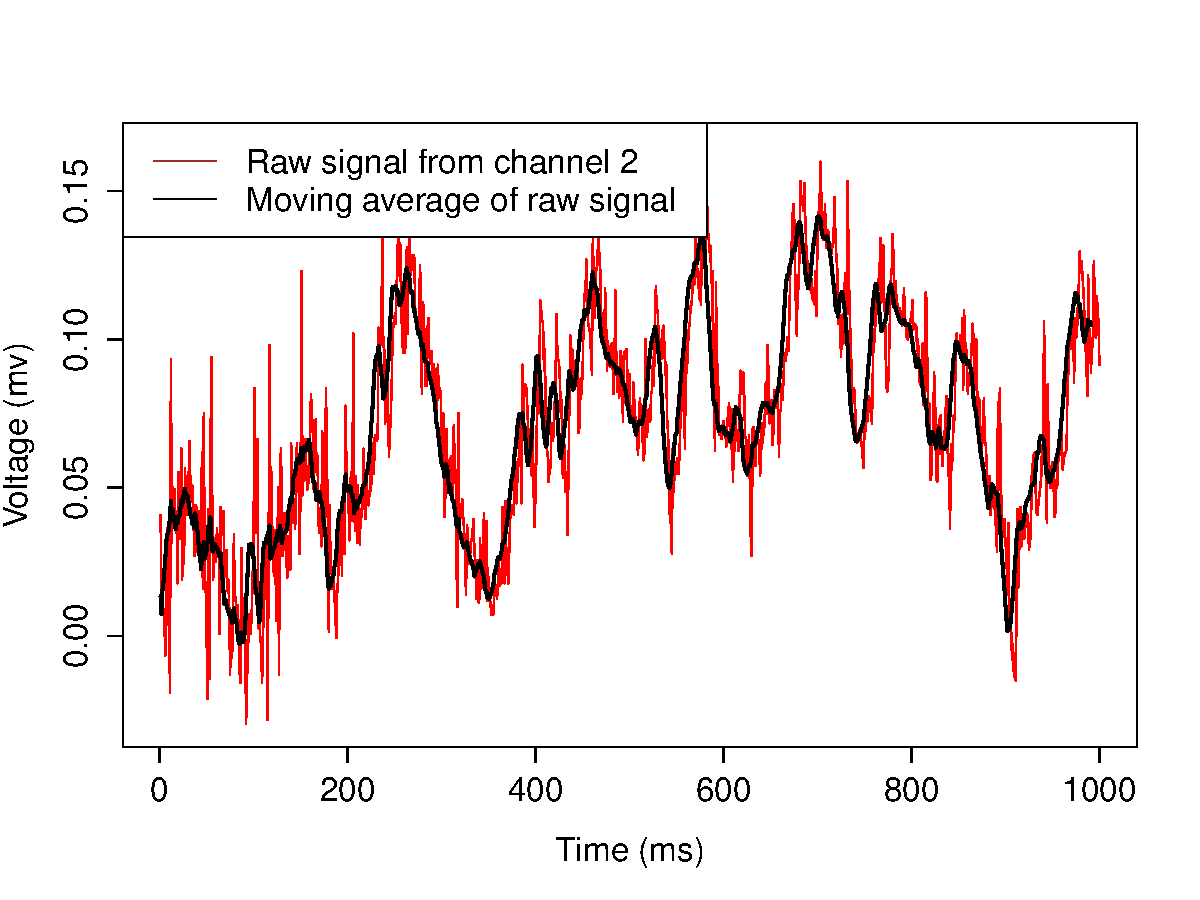
\includegraphics[width=0.95\linewidth]{figures/sample_moving_average.pdf}
%   \caption{A moving average line fitted through the first second ($10^3$ data points) of channel 2. A rolling window of 10 is used.}
%   \label{fig:spline_sample}
% \end{figure}

% \subsecttion of the signal calculated from the signal's Fourier transform as used by Nes \textit{et al.} \cite{Nes2015}\cite{Takens1981}.

\subsection{Implementation}
\subsubsection{Data Preprocessing}
Some of our edge weights had some Not A Numerical (\textit{NaN}) values, and those were altered to 0, which is the lowest $\rho$ score possible. Once that error was corrected and the data has been put in the graph series format, separated into the three different datasets, we perform Principal Component Analysis (PCA) to reduce the dimensionality of the datasets. This both gives us insight into what components of the graph are logically important for the model and helps decrease the time required to run our model. The results of PCA was used to create three different datasets from each dataset: a dataset that covered 80\% of the variance, a dataset that covered 90\% of the variance, and a dataset that covered 99\% of the variance. This was done to test how dimensionality reduction would affect the final clustering efforts. Furthermore, there were some edges that showed a consistent weight of 0 (for example, all edges from node 2 to node 1 were of weight 0), and having that redundant data is not helpful to distinguishing states. PCA would help us remove such unvarying features from the datasets.

 If the scoring for the reduced datasets with only 80\% of the variance is similar to the scoring of the reduced datasets with 99\% of the variance, then we use the less dimensional reduced datasets even though they give us a less accurate version of the original information. The original dimensionality of the datasets was 132 features per data point, and a list of the PCA datasets and their different variance levels with component numbers are reported in table \ref{tab:pca_datasets}. After the principal component analysis was done on the datasets, the components required to reach the threshold levels of 80, 90, and 99 percents were recorded in table \ref{tab:components_needed_for_variance} (Fig. \ref{fig:pca_analysis_variance}).


\begin{table}[H]
\centering
\caption{Dataset names for the result of PCA analysis. Three different reduced datasets are produced each of which keeps a certain percentage of the original variance. Since we started with three datasets and created three new ones out of each by applying PCA with different levels of components, we arrive at 9 total reduced datasets.}
\label{tab:pca_datasets}
\begin{tabular}{|c|c|c|c|}
\hline
  &  80\% variance &  90\% variance & 99\% variance \\ \hline
 
dataset 50 & reduced 50 80 & reduced 50 90 & reduced 50 99  \\ \hline
dataset 200 & reduced 200 80 & reduced 200 90 & reduced 200 99  \\ \hline
dataset 250 & reduced 250 80 & reduced 250 90 & reduced 250 99  \\ \hline
\end{tabular}
\end{table}


\begin{figure}[H]
  \centering
  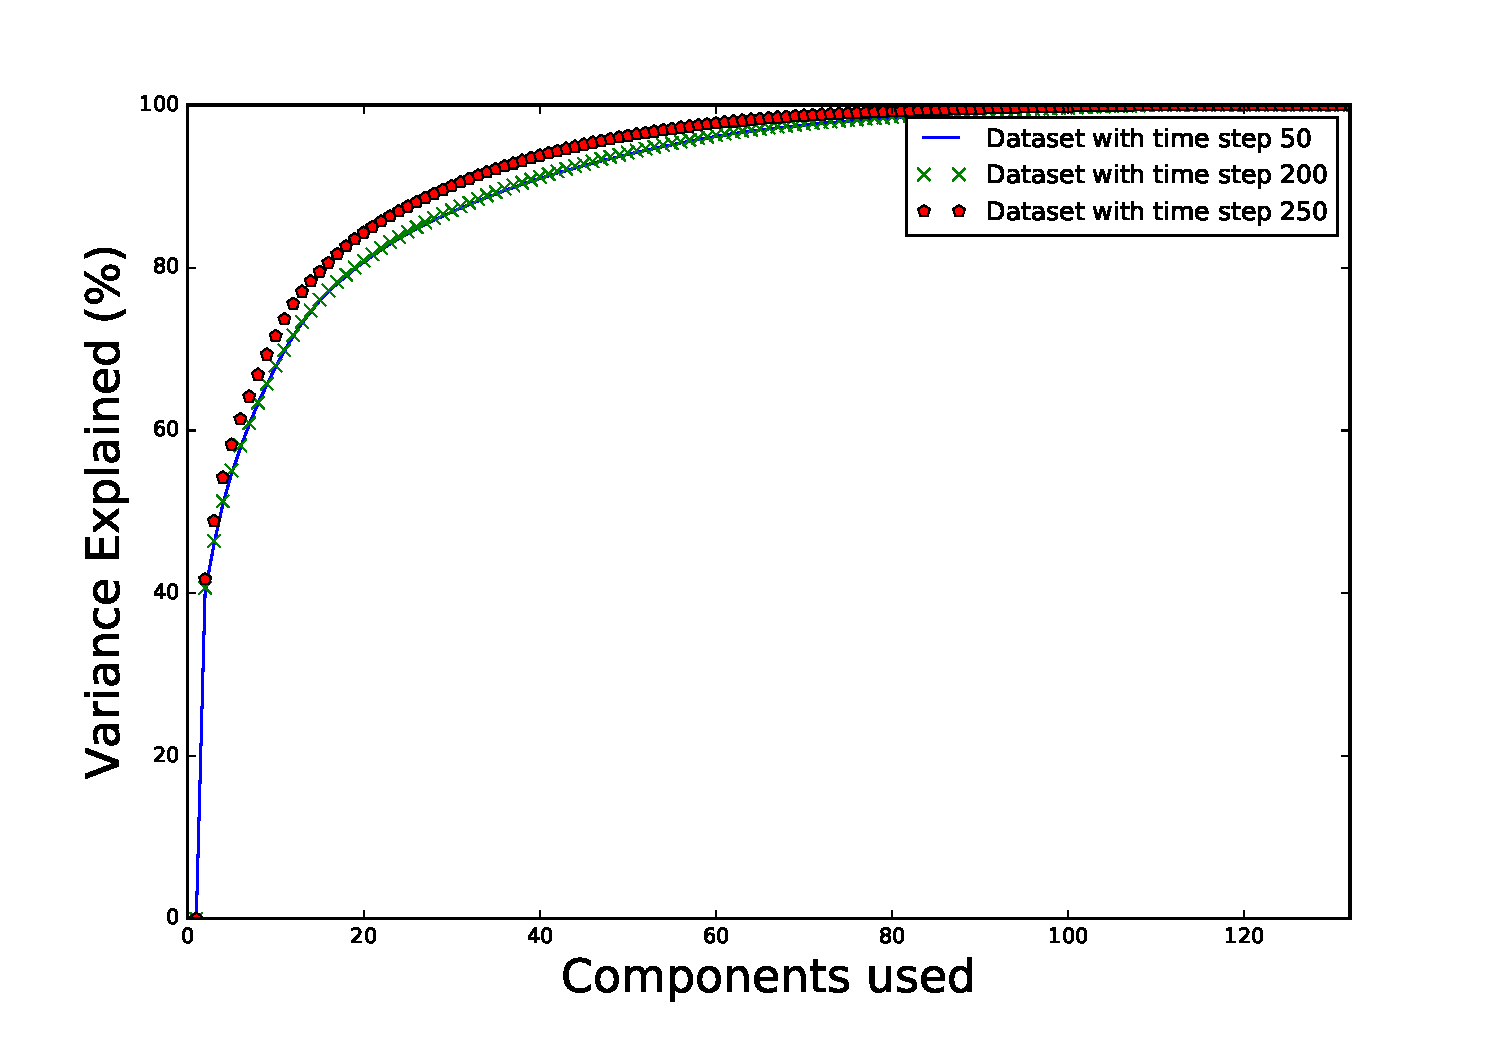
\includegraphics[width=0.55\linewidth]{figures/variance_explained_with_pca.pdf}
  \caption{Principle Component Analysis conducted on the three datasets reveals that the overall variance of the data can be maintained by using only a subset of the edges of the graph rather than all of them. The dataset with a time step of 250 ms needs less components to explain the variance than the other two, while the datasets with 200 and 50 ms time steps showed an almost exact level of variance explained with the number of components. This suggests that the 250 ms dataset is not complex enough, which might indicate that 2000 ms is too big of a time frame to record the granular communication speed of the brain.}
  \label{fig:pca_analysis_variance}
\end{figure}

\begin{table}[H]
\centering
\caption{Different component numbers are needed for each dataset to maintain a certain level of variance explained using PCA for dimensionality reduction. These values for components required for reaching a score standard were used to produce reduced forms of the datasets as noted in table \ref{tab:pca_datasets}. These reduced forms of the datasets were then analyzed in figure \ref{fig:silhouette_scores}.}
\label{tab:components_needed_for_variance}
\begin{tabular}{|c|c|c|c|}
\hline
 &  80\% variance explained &  90\% variance explained & 99\% variance explained \\ \hline
 
 Components in dataset 50 & 20 &  38&  87  \\ \hline
 Components in dataset 200 & 20 &  37&  87\\ \hline
 Components in dataset 250 & 16 &  30&  76  \\ \hline
\end{tabular}
\end{table}



\subsubsection{Clustering}
Once the dimensionality of the data was reduced with PCA, a Gaussian Mixture clusterer was initiated for each dataset from table \ref{tab:pca_datasets}, and all number of clusters from $2$ to $40$ were tried and tested by the Silhouette Coefficient and Calinsky-Harabaz Index scorers (Figs. \ref{fig:silhouette_scores}, \ref{fig:calinsky_scores}).

The complete ordered list of procedures was:
\begin{itemize}
  \item Removing NaN's with 0's if any exist in the edge weights
  \item Splitting the dataset into three datasets depending on the time step used
  \item Vectorizing the graphs so that each graph is a data point
  \item Running PCA analysis on the three datasets with varying degree of variance kept, creating 9 total datasets
  \item Clustering the PCA-reduced datasets with cluster numbers from 2 to 40.
  \item Computing Silhouette and Calinsky scores on the clusters in the previous step
\end{itemize}

The procedures were implemented successfully, but computing the silhouette and Calinsky scores was a bottleneck as it required calculating the distances between each data point. This could possibly have been avoided by pre-calculating the distances between all data points and passing them to the silhouette and Calinsky scoring functions, a feature available in the sci-kit learn library.

\begin{figure}[H]
  \centering
  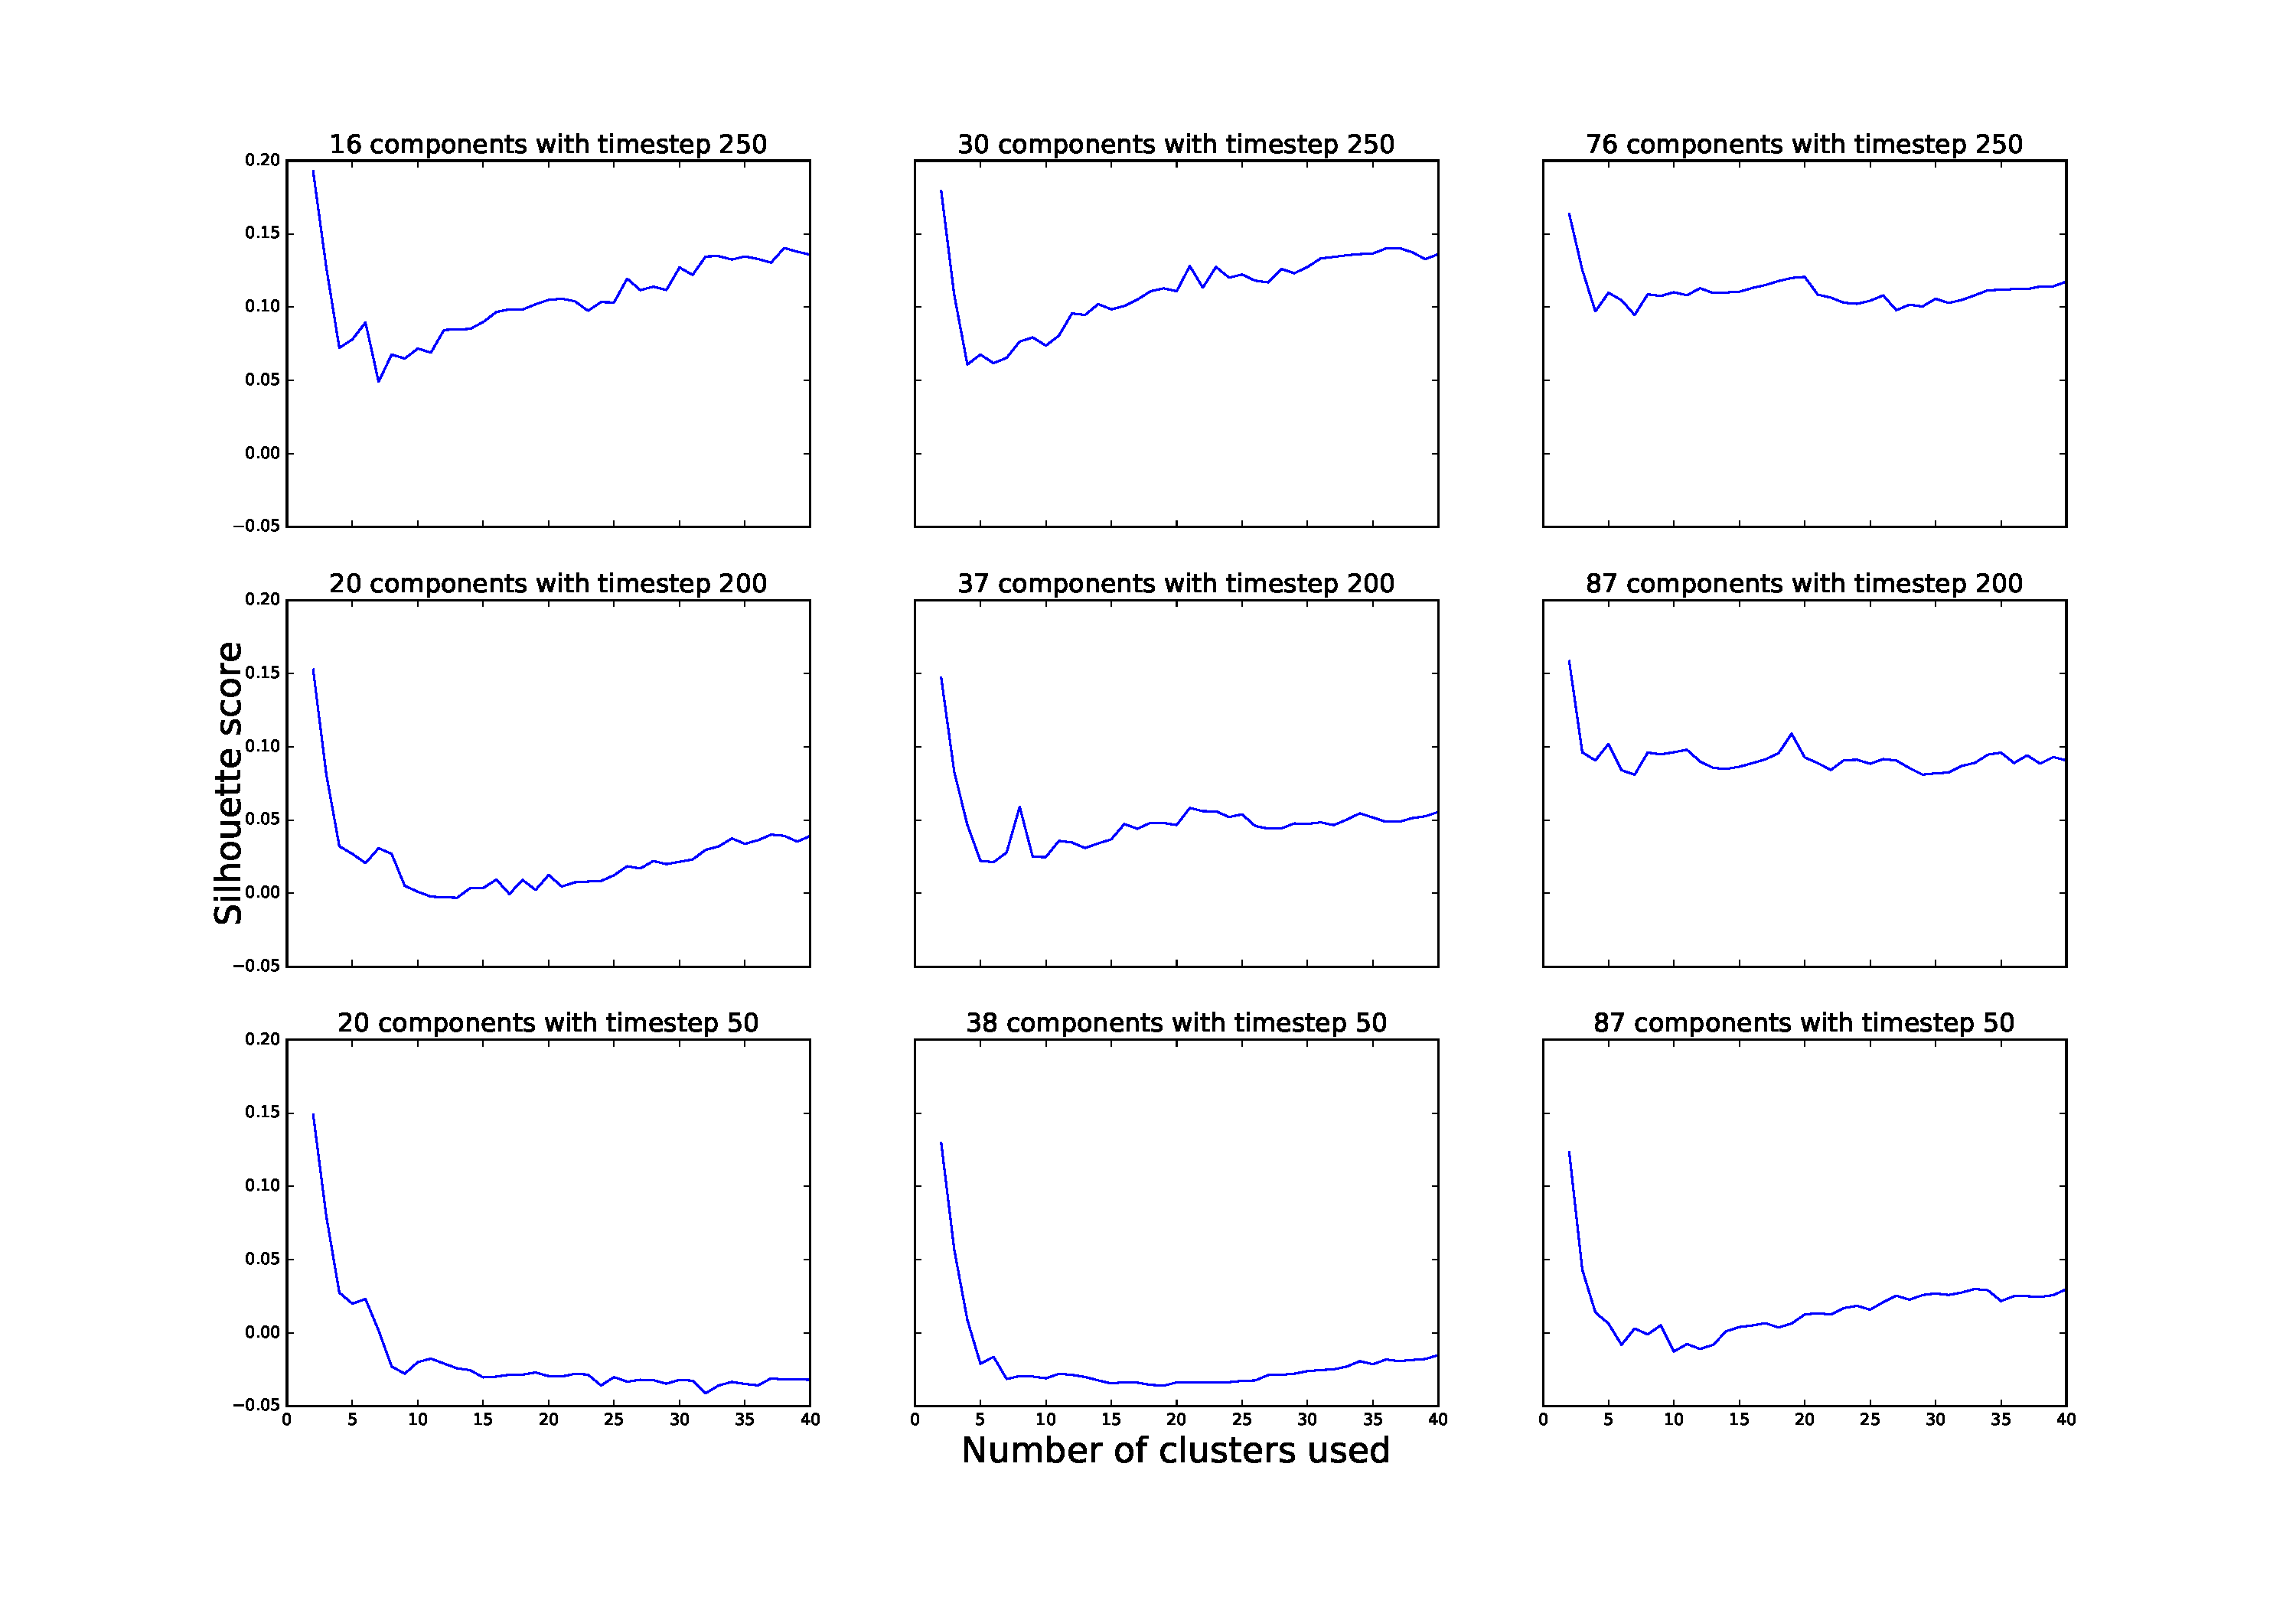
\includegraphics[width=\linewidth]{figures/silhouette_scores.pdf}
  \caption{Silhouette scores for clustering with different cluster numbers. Scores close to 1 suggest clusters that are dense and well separated; scores close to -1 suggest clusters that overlap and are not dense. The best score is consistently when there are only two clusters, and dips greatly when creating more clusters but begins to rise after ~30 clusters. With the dataset 250 and dataset 50, PCA with less components (16 and 20 components respectively) showed a better silhouette score than the other, higher component reduced datasets. However, dataset 200 showed a better silhouette score when more components were used. Especially with a rather thin margin of difference in scores between components, it is difficult to conclude whether having more PCA reductionist approach is beneficial.}
  \label{fig:silhouette_scores}
\end{figure}



\begin{figure}[H]
  \centering
  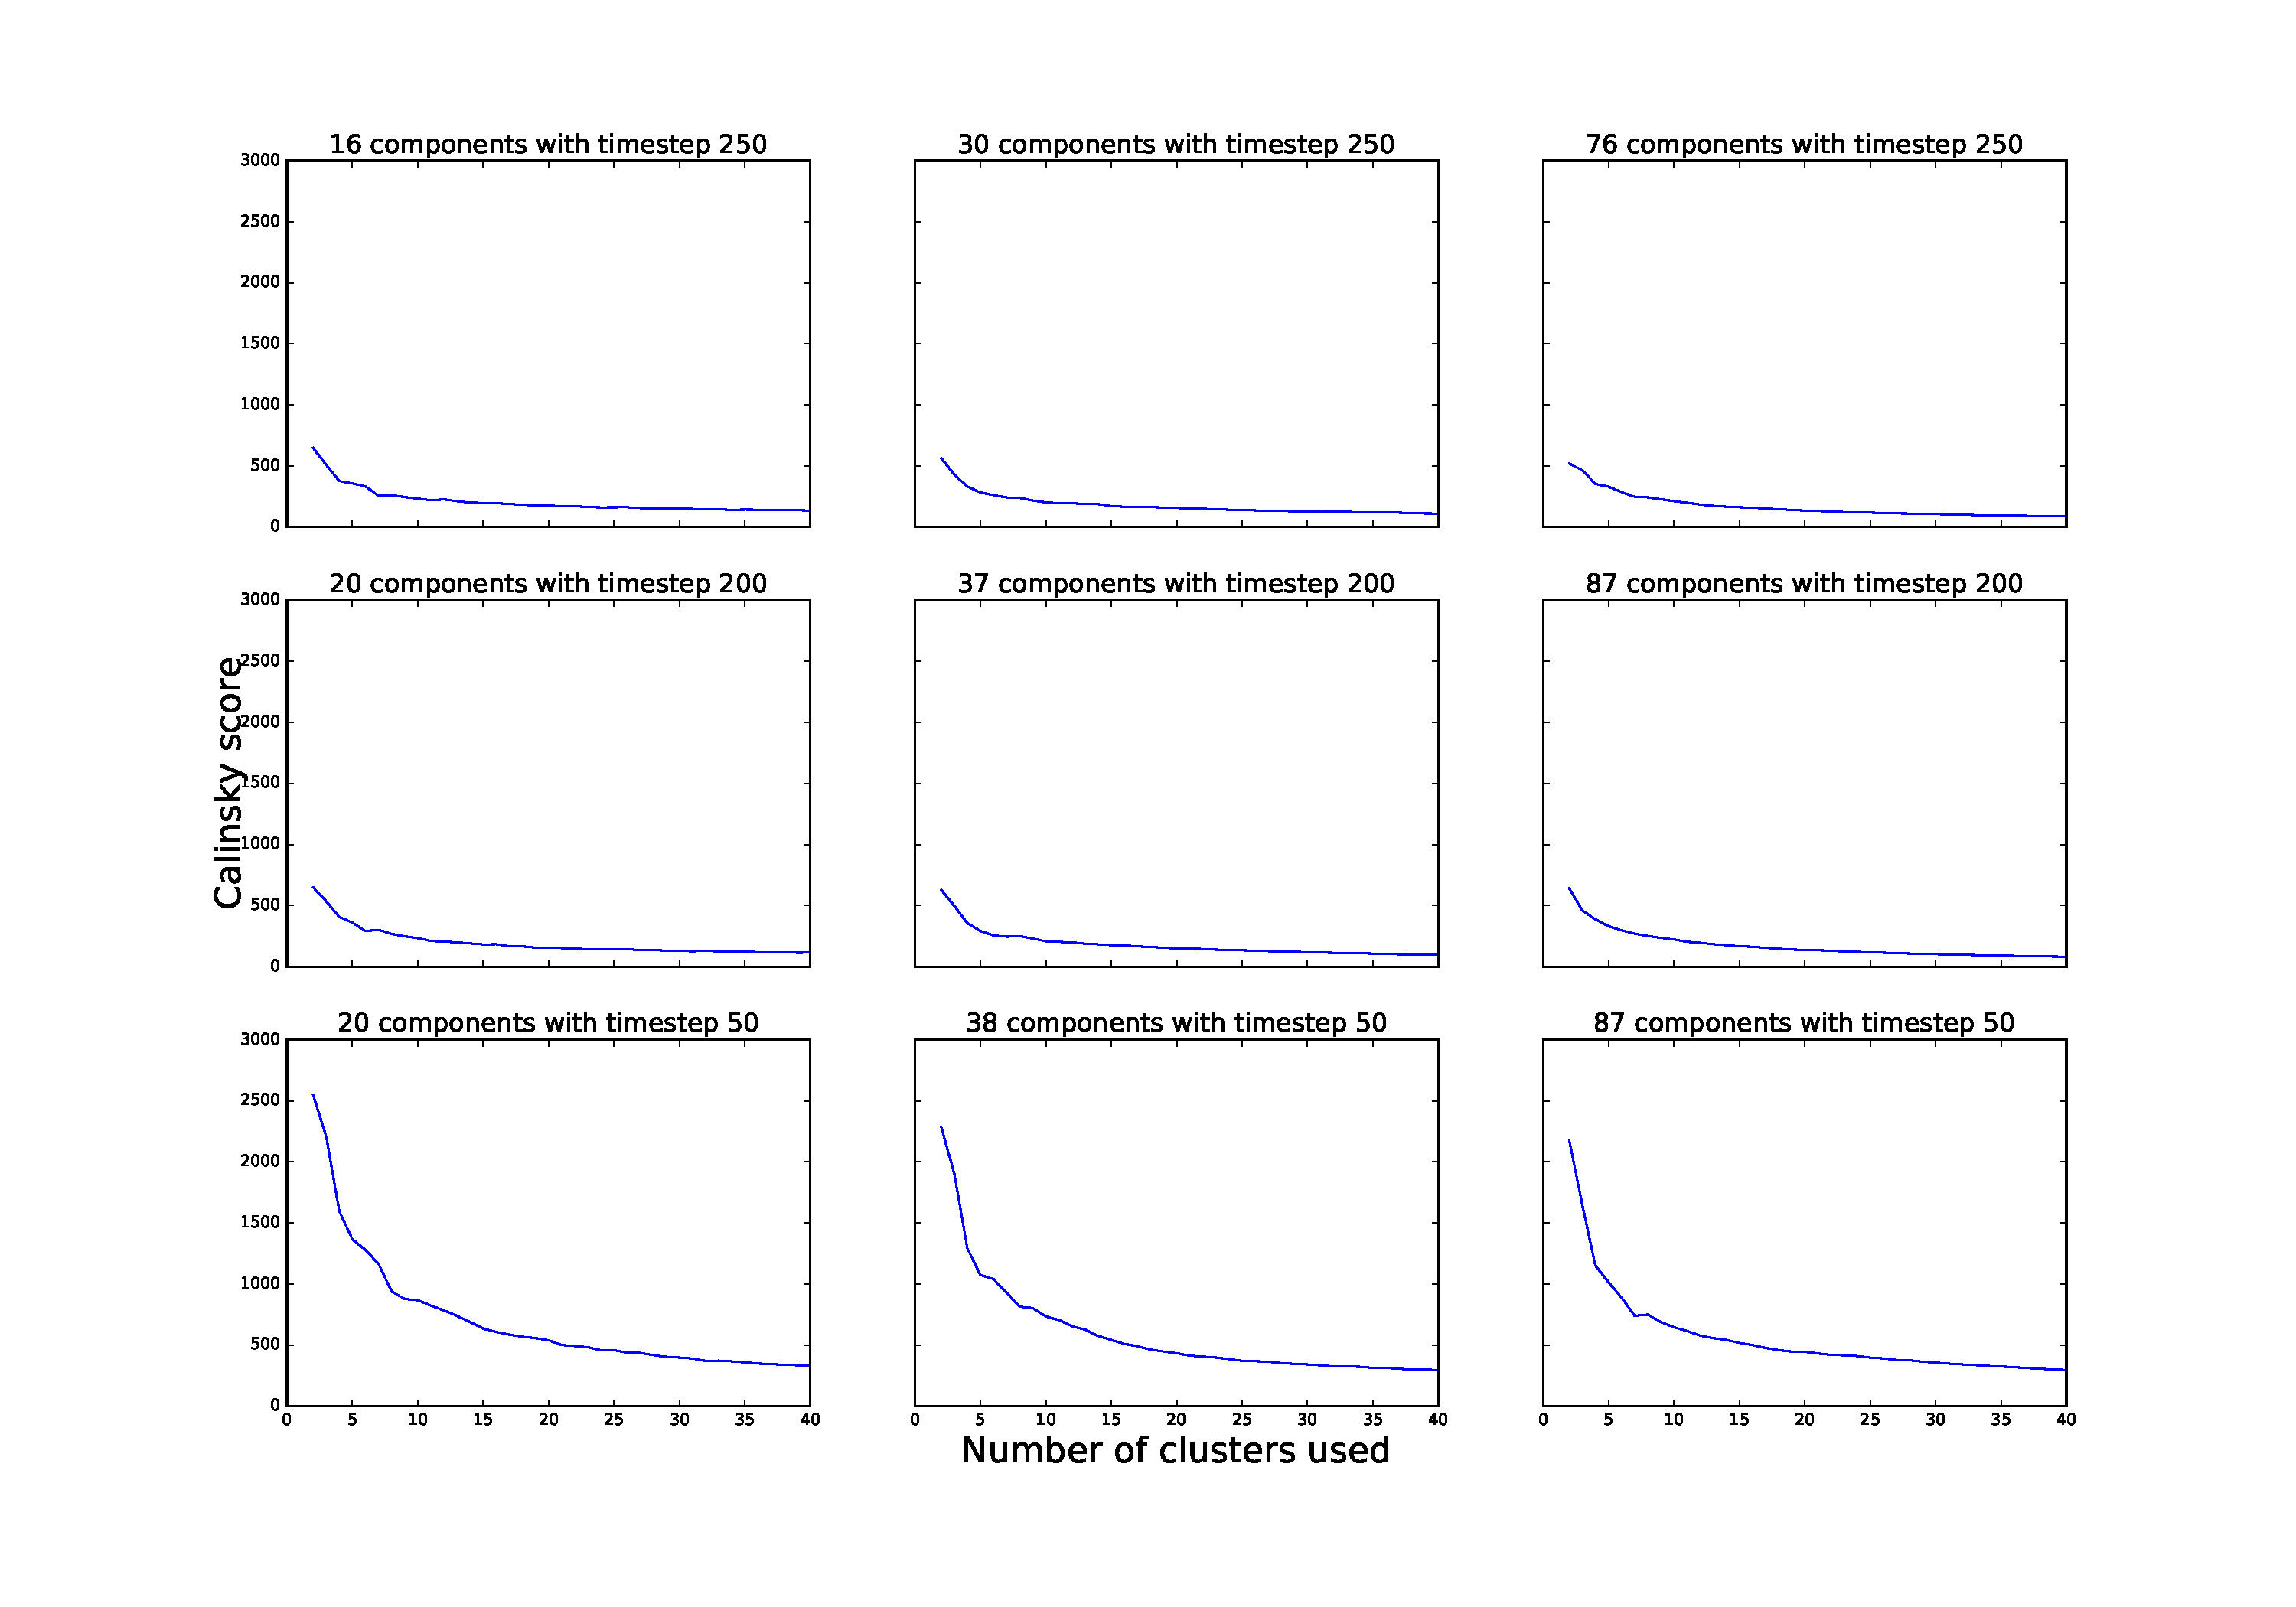
\includegraphics[width=\linewidth]{figures/calinsky_scores.pdf}
  \caption{Calinsky-Harabaz scores for clustering with different cluster numbers. Higher scores mean more separated and dense clusters, which is positive. The score dips greatly when creating more than two clusters, but begins to rise after ~30 clusters. The silhouette scores show that having more components when reducing with PCA results in better clustering scores. The scores also show that scores for the reduced data that keep 99\% of the variance (right column) are all similar in score and trend.}
  \label{fig:calinsky_scores}
\end{figure}

From figures \ref{fig:silhouette_scores} and \ref{fig:calinsky_scores}, it can be seen that the best clustering number is two, and it happens with dataset \textit{reduced 50 80} (dataset that is made with time step of 50 and transformed with PCA). We therefore fine tuned a Gaussian Mixture model with the \textit{reduced 50 80} dataset using Grid Search as implemented by the scikit learn library. The silhouette score was used as a scoring function for the grid search performance measurement. The parameters tuned with grid search was the \textit{covariance type} (with a choice of tied, diagonal, sphere, or full), and the best parameter was 'tied' with a silhouette score of $0.254$. This is an increase of 0.05 in the silhouette score, which is a ~25\% improvement.

\subsection{Results}

The results so far indicate that the rat's brain showed the presence of two distinct brain states, as we can cluster the brain's communication network into two clusters. This could be good news, since we can assume that the two brain states are \textit{epilepsy state} and \textit{normal state}. This simplifies our choice of metric to evaluate the model since we can use a simple F1 measurement by assuming the less frequent brain state is the epileptic state, and record the less occurring cluster as the epileptic cluster; we then test the time indicies of this cluster with the time indicies we were given for when epilepsy was evoked. Since we know that the epilepsy happened between seconds 447-457 and 250-260, we set true labels to be $0$ for all data points that were in that time period, and $1$ for all other data points. We then set the less frequent cluster to be of label $0$ (epilepsy cluster) and the more frequent cluster to $1$ (non-epilepsy cluster). Our evaluation metric then becomes the F1 score of the predicted labels against the true labels that we produced given the knowledge of our experiment.

Using the fine-tuned model, we achieve an F1 score of 0.788, which seems acceptable at first, but is rather disappointing when considering that the blind benchmark discussed in section \ref{sec:benchmark} has a score of 0.99. This is mainly due to the fact that the epilepsy state is infrequent, and so a clustering of non-epilepsy state as epilepsy creates a great error. This indicates that our model does not perform better than blindly guessing that there is only one state in the brain. This does not align with our hopes and expectations for the clustering solution. 

To analyze what our model is doing, we plot an annotated time strip that shows what each time window of causality was clustered to (Fig. \ref{fig:strip_visual}). From this graph, it can be seen that there is no correlation between what we observe in the real-life experiment and our clustering on the graph series constructed from Sugihara Causality measures. 

\begin{figure}[H]
  \centering
  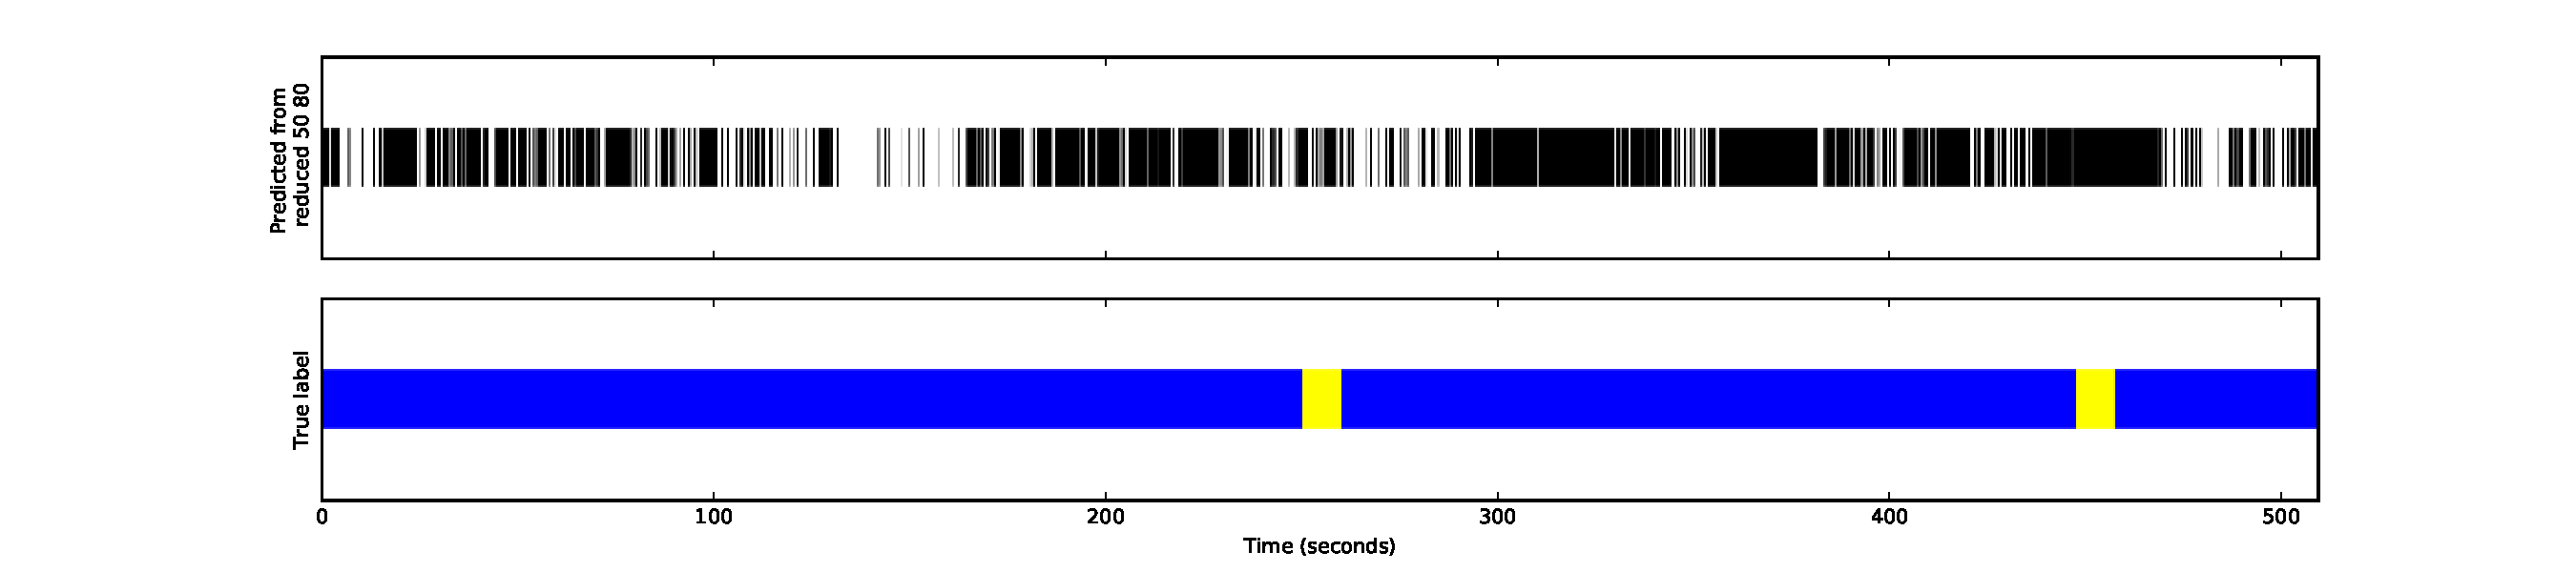
\includegraphics[width=\linewidth]{figures/strip_visual.pdf}
  \caption{Time strips that show the epilepsy time track and the results of the respective clustering done on the Sugihara Causality graphs from those time windows. Blue corresponds to true non-epileptic state; yellow to true epileptic state; white to predicted epileptic state; and black to predicted non-epileptic state. There are only two clusters in the top bar. The clustering results does not show any correlation with the actual epilepsy induction time series.}
  \label{fig:strip_visual}
\end{figure}


\subsection{Discussion}
Initial analysis shows that the causality network is very dense with highly weighted edges. The high density of the graph could have been a side effect of Sugihara's model ability to detect downstream causality. If that is the case, then many of the causal connections detected could in fact be residuals of upstream interactions in the brain network. Put in another way, if region A of the brain was causing region B to fire, and region B causes region C to fire, then the Sugihara causality model would report a causality measure between A and C. Downstream causality measures can be detected by observing both the magnitude of the cross map skill as well as the time lag that produces the greatest cross map skill (Fig. 3 in \cite{Ye2015}). Although we could have used this method in our experiment to remove the possibility of picking up extra weights from downstream causality, initial trials showed that the computational power required for that analysis were greater than the capacity available at UCCS. 

Concerning the high possibility of the presence of unidirectional forcing from figure \ref{fig:diff_within_pair_hist}, Ye \textit{et al.} showed unidirectional forcing can be untangled by inspecting the greatest time lag of the two that produces the highest causality measure (Fig. 2 in \cite{Ye2015}). In order to allay the problem of unidirectional forcing, the best lag of each pair is considered. This is a tricky problem because there is no clear range for which to test the lag. This is because the time delay for neuronal activity is yet studied, and how that translates to EEG data could be tricky. We reserve the use of this method due to its computational complexity which would add to the already high time complexity of the analysis.

The theoretical implications of this model could present a novel representation of information flow in the brain and determining causality within the brain. If the graph output of this method id reliable, it could help outline information flow within the brain, much like one would observe in a magnetic wave flowing through an fMRI recording. 



\subsection{Future Work}

Since various improvements can be made to this work, we break it down by stage of implementation.

\subsubsection{Methods}
It would have been enriching to our knowledge of our true labels if we had access to exactly what the rat was doing during the experiment. A video capture of the rat, or recorded structured interventions to the rat's behavior could have provided more opportunity to label the data with ground truth. For example, we could have shone light into the rat's eyes, and recorded that as a separate brain state; we could have put the rat on a hamster wheel and recorded his running as a separate brain state; eating food could be a brain state; and sleeping is another possible brain state. All these interventions to the rat's environment could enable us to gain more labels rather than the simple epilepsy, non-epilepsy labeling system we worked with. Although this complicates our approach, it would allow us access to better scoring metrics other than the silhouette and Calinksy-Harabaz scores, where the labels have to be known.

\subsubsection{Sugihara Causality Network}
Future work in this area could focus on verifying this model through controlled experiments. Such experiments could be in the form of stimulating a part of the brain (e.g. shining strong light on an the eye to excite the visual cortex) and observing the model's behavior. One would expect a high value of out degrees from the specific region during such an experiment, as it attempts to convey a considerable portion of information to the rest of the brain. Moreover, a clear proof should be presented as to what the most reliable time window and step size ought to be when producing the causality graphs. Such a task can be done by measuring graph similarity of the same time segment as the time window gets shortened incrementally.

\subsubsection{Data Processing}
Apart from collecting the data and applying Sugihara Causality on the dataset (which took 2 days), calculating the current source density using kCSD was by far the most time consuming process. Even though we do not discuss the details of how that was done in this project (we provide already processed kCSD data), it would have been nice to see a GPU implementation of the kCSD, which took advantage of CPU parallelism but not GPU parallelism. This would massively improve the speed of the implementation and allow for testing more various approaches in the Sugihara Causality step. 

\subsubsection{Cluster Scoring with Higher Dimensions}
Due to the high dimensionality of the dataset we worked with, it was difficult to visually measure how well the clustering with different number of clusters took place. Beyond three dimensions, it is impossible to visualize the dataset with labels, and although the PCA reduction resulted in a greatly reduced dimensional feature, it was not enough to allow us to visualize the clusters visually.
Following the assumption that downstream causality decreases in magnitude as it travels downstream in the network, we can use this to traverse the graph and rid of any paths that decreases in causality as it goes downstream.

\subsection{Conclusion}
The experiment we conduscted transformed 32 EEG electrode signals into 12 regional neuronal activity signals, and created a (theoretical) communication network from those signals using Sugihara Causality. These communication graphs were analyzed by unsupervised learning using the Gaussian Mixture model for the goal of gaining some insight into the epileptic state, and test whether unsupervised clustering is able to discriminate between brain states from the communication networks. From our initial results, it is clear that our approach is not successful in distinguishing brain states in a rat's brain. However, the ground work has been laid for future explorations in the topic of communication networks in the brain. 
